%!TEX root = ../dissertation.tex
\begin{savequote}[75mm]
“How well we communicate is determined not by how well we say things, but how well we are understood.” 
\qauthor{Andrew Grove}
\end{savequote}

\chapter{Planificación, análisis y diseño}
\chapter*{Planificación}
A continuación se expone mediante un \textcolor{SchoolColor}{diagrama de Gantt} como se ha distribuido el tiempo durante estos 5 meses para cada tarea de este proyecto, a partir de mediados de Julio hasta la segunda semana de Diciembre.
\\[\baselineskip]
%\\[\baselineskip]
\setganttlinklabel{f-s}{FINISH-TO-START}
\begin{figure}[H]
 \makebox[\textwidth][c]{
\begin{ganttchart}[ vgrid,x unit=0.4cm,
            y unit title=0.7cm,
            y unit chart=0.9cm,
            canvas/.append style={rounded corners=1mm, draw=none, fill=orange!9},
            bar/.append style={fill=orange!40,rounded corners=1.5mm, draw=none},
            milestone/.append style={fill=orange!90,rounded corners=0mm, draw=none},
            link/.append style={-to,black!70},
            title/.style={fill=orange!60, draw=none, rounded corners=2mm},
title label font=\color{white}\bfseries,
title left shift=-.1,
title right shift=-.1,
title top shift=.05,
title height=.75
]{1}{30}
\gantttitle{2016}{30} \\
%\gantttitlelist{1,...,6}{5} \\
\gantttitle{Julio}{5}
\gantttitle{Agosto}{5}
\gantttitle{Septiembre}{5}
\gantttitle{Octubre}{5}
\gantttitle{Noviembre}{5}
\gantttitle{Diciembre}{5} \\
%\ganttgroup{Group 1}{1}{7} \\
\ganttbar{Revisión bibliográfica y documentación}{3}{9} \\
\ganttmilestone{Fin de bibliografía}{9} \ganttnewline
\ganttlinkedbar[link type=f-s]{Análisis de requisitos y diseño}{10}{10}\\
\ganttlinkedbar[link type=f-s]{Implementación y eval. Del Tokenizador}{11}{15}\\
\ganttlinkedbar[link type=f-s]{Implementación y eval. Del POS Tagger}{16}{20}\\
\ganttlinkedbar[link type=f-s]{Implementación y eval. Del Lematizador}{21}{25}\\
\ganttmilestone{Fin de código}{25} \ganttnewline
\ganttlinkedbar{Memoria}{26}{27}\\
%\ganttlinkedbar[link type=f-s]{Interfaz gráfica}{19}{23}\\
%\ganttmilestone{Informe trimestral 2}{24} \ganttnewline
%\ganttlinkedbar{Interfaz gráfica}{23}{29}\\
%\ganttlinkedbar{Entrega final}{29}{30}\\
\ganttlink{elem0}{elem1}
\ganttlink{elem5}{elem6}
\end{ganttchart}}
\end{figure} 

\chapter*{Análisis de requisitos}
En esta sección se muestra la especificación de requisitos para el proyecto de manera formal, a través de plantillas que muestran información relevante del requisito, como la descripción, su prioridad, estado o riesgo. Al ser demasiados, se exponen solo los más importantes.
\subsection*{requisitos funcionales}
%\usepackage{array}
\newcolumntype{L}{>{\arraybackslash}m{15cm}}
%RF 1
\begin{table}[H]
%\caption{My caption}
\label{my-label}
\begin{tabular}{|l|l|l|l|l|l|l|}
\hline
\multicolumn{7}{|l|}{\textcolor{SchoolColor}{Identificador:} RF-01}                                 \\ \hline
\multicolumn{4}{|l|}{\textcolor{SchoolColor}{Necesidad:} Alta} & \multicolumn{3}{l|}{\textcolor{SchoolColor}{Autor:} Cristina Heredia}         \\ \hline
\multicolumn{7}{|L|}{\textcolor{SchoolColor}{Descripción:} El sistema incluirá un método de parseado de texto, al que el usuario  especificará una cadena de texto y cual de las tres tareas desea realizar(tokenizado, etiquetado,lematización) mediante parámetros booleanos. Devuelve el resultado de aplicarle al texto especificado la acción solicitada. Si no se especifica opción, devuelve el texto tal como lo especificó el usuario.  }                                 \\ \hline
\multicolumn{4}{|l|}{\textcolor{SchoolColor}{Prioridad: }Alta} & \multicolumn{3}{l|}{\textcolor{SchoolColor}{Riesgo:} Medio}         \\ \hline
\multicolumn{5}{|l|}{\textcolor{SchoolColor}{Dependencias: }RF-02, RF-03, RF-07}         & \multicolumn{2}{l|}{\textcolor{SchoolColor}{Estado:} Hecho} \\ \hline
\end{tabular}
\end{table}
%RF 2
\begin{table}[H]
%\caption{My caption}
\label{my-label}
\begin{tabular}{|l|l|l|l|l|l|l|}
\hline
\multicolumn{7}{|l|}{\textcolor{SchoolColor}{Identificador:} RF-02}                                 \\ \hline
\multicolumn{4}{|l|}{\textcolor{SchoolColor}{Necesidad:} Alta} & \multicolumn{3}{l|}{\textcolor{SchoolColor}{Autor:} Cristina Heredia}         \\ \hline
\multicolumn{7}{|L|}{\textcolor{SchoolColor}{Descripción:} El sistema incluirá un método de procedimiento de tokenización de texto, que separará el texto en sus unidades mínimas; los tokens. Si el texto contiene emoticonos, los cambia por el sentimiento que tengan asociado. Recibe como parámetro una cadena de texto especificada por el usuario. Devuelve una lista de listas de tokens, donde cada lista de tokens se corresponde con una frase del texto del usuario. }                                 \\ \hline
\multicolumn{4}{|l|}{\textcolor{SchoolColor}{Prioridad: }Alta} & \multicolumn{3}{l|}{\textcolor{SchoolColor}{Riesgo:} Medio}         \\ \hline
\multicolumn{5}{|l|}{\textcolor{SchoolColor}{Dependencias: }}         & \multicolumn{2}{l|}{\textcolor{SchoolColor}{Estado:} Hecho} \\ \hline
\end{tabular}
\end{table}

%RF 3
\begin{table}[H]
%\caption{My caption}
\label{my-label}
\begin{tabular}{|l|l|l|l|l|l|l|}
\hline
\multicolumn{7}{|l|}{\textcolor{SchoolColor}{Identificador:} RF-03}                                 \\ \hline
\multicolumn{4}{|l|}{\textcolor{SchoolColor}{Necesidad:} Alta} & \multicolumn{3}{l|}{\textcolor{SchoolColor}{Autor:} Cristina Heredia}         \\ \hline
\multicolumn{7}{|L|}{\textcolor{SchoolColor}{Descripción:} El sistema incluirá un método de etiquetado morfosintáctico de texto (POS Tagger), que etiquetará cada palabra(token) con su categoría morfosintáctica según el léxico, una morfología y un contexto que recibirá como parámetro.  También recibe como parámetro una lista con los tokens del texto introducido por el usario, por lo tanto requiere de una tokenización previamente. Devuelve una lista de pares (token,etiqueta).  }                                 \\ \hline
\multicolumn{4}{|l|}{\textcolor{SchoolColor}{Prioridad: }Alta} & \multicolumn{3}{l|}{\textcolor{SchoolColor}{Riesgo:} Medio}         \\ \hline
\multicolumn{5}{|l|}{\textcolor{SchoolColor}{Dependencias: }RF-02,RF-04,RF-05, RF-06}         & \multicolumn{2}{l|}{\textcolor{SchoolColor}{Estado:} Hecho} \\ \hline
\end{tabular}
\end{table}

%RF 4
\begin{table}[H]
%\caption{My caption}
\label{my-label}
\begin{tabular}{|l|l|l|l|l|l|l|}
\hline
\multicolumn{7}{|l|}{\textcolor{SchoolColor}{Identificador:} RF-04}                                 \\ \hline
\multicolumn{4}{|l|}{\textcolor{SchoolColor}{Necesidad:} Alta} & \multicolumn{3}{l|}{\textcolor{SchoolColor}{Autor:} Cristina Heredia}         \\ \hline
\multicolumn{7}{|L|}{\textcolor{SchoolColor}{Descripción:} El sistema incluirá un método de aplicación de un contexto a una lista de tokens ya etiquetados morfosintácticamente, para mejorar el etiquetado de los mismos. Como resultado devuelve una lista con los tokens y sus nuevas etiquetas, en un par (token,tag).}                                 \\ \hline
\multicolumn{4}{|l|}{\textcolor{SchoolColor}{Prioridad: }Alta} & \multicolumn{3}{l|}{\textcolor{SchoolColor}{Riesgo:} Medio}         \\ \hline
\multicolumn{5}{|l|}{\textcolor{SchoolColor}{Dependencias: } RF-02, RF-05}         & \multicolumn{2}{l|}{\textcolor{SchoolColor}{Estado:} Hecho} \\ \hline
\end{tabular}
\end{table}

%RF 5
\begin{table}[H]
%\caption{My caption}
\label{my-label}
\begin{tabular}{|l|l|l|l|l|l|l|}
\hline
\multicolumn{7}{|l|}{\textcolor{SchoolColor}{Identificador:} RF-05}                                 \\ \hline
\multicolumn{4}{|l|}{\textcolor{SchoolColor}{Necesidad:} Alta} & \multicolumn{3}{l|}{\textcolor{SchoolColor}{Autor:} Cristina Heredia}         \\ \hline
\multicolumn{7}{|L|}{\textcolor{SchoolColor}{Descripción:} El sistema incluirá un método de creación de un diccionario de léxico, a partir de la lectura y manipulación de un fichero de 85877 líneas de reglas léxicas. Éste será usado en el POS tagger para realizar un etiquetado inicial. }                                 \\ \hline
\multicolumn{4}{|l|}{\textcolor{SchoolColor}{Prioridad: }Alta} & \multicolumn{3}{l|}{\textcolor{SchoolColor}{Riesgo:} Medio}         \\ \hline
\multicolumn{5}{|l|}{\textcolor{SchoolColor}{Dependencias: } }         & \multicolumn{2}{l|}{\textcolor{SchoolColor}{Estado:} Hecho} \\ \hline
\end{tabular}
\end{table}

%RF 6
\begin{table}[H]
%\caption{My caption}
\label{my-label}
\begin{tabular}{|l|l|l|l|l|l|l|}
\hline
\multicolumn{7}{|l|}{\textcolor{SchoolColor}{Identificador:} RF-06}                                 \\ \hline
\multicolumn{4}{|l|}{\textcolor{SchoolColor}{Necesidad:} Alta} & \multicolumn{3}{l|}{\textcolor{SchoolColor}{Autor:} Cristina Heredia}         \\ \hline
\multicolumn{7}{|L|}{\textcolor{SchoolColor}{Descripción:} El sistema incluirá un proceso de aplicación  de reglas morfológicas a un token dado con una etiqueta dada, que se reciben como parámetros. Ésto sirve de nuevo para mejorar el etiquetado, esta vez teniendo en cuenta la morfología. }                                 \\ \hline
\multicolumn{4}{|l|}{\textcolor{SchoolColor}{Prioridad: }Alta} & \multicolumn{3}{l|}{\textcolor{SchoolColor}{Riesgo:} Medio}         \\ \hline
\multicolumn{5}{|l|}{\textcolor{SchoolColor}{Dependencias: }RF-02, RF-05 }         & \multicolumn{2}{l|}{\textcolor{SchoolColor}{Estado:} Hecho} \\ \hline
\end{tabular}
\end{table}

%RF 7
\begin{table}[H]
%\caption{My caption}
\label{my-label}
\begin{tabular}{|l|l|l|l|l|l|l|}
\hline
\multicolumn{7}{|l|}{\textcolor{SchoolColor}{Identificador:} RF-07}                                 \\ \hline
\multicolumn{4}{|l|}{\textcolor{SchoolColor}{Necesidad:} Alta} & \multicolumn{3}{l|}{\textcolor{SchoolColor}{Autor:} Cristina Heredia}         \\ \hline
\multicolumn{7}{|L|}{\textcolor{SchoolColor}{Descripción:} El sistema incluirá un proceso de lematización que obtendrá la forma base de la palabra, aplicando un diccionario y varios algoritmos. 
Requiere de un etiquetado previo de las palabras, por lo que recibe como argumento una lista de (palabra,etiqueta) y devuelve una lista de (palabra,etiqueta,lema). }                                 \\ \hline
\multicolumn{4}{|l|}{\textcolor{SchoolColor}{Prioridad: }Alta} & \multicolumn{3}{l|}{\textcolor{SchoolColor}{Riesgo:} Medio}         \\ \hline
\multicolumn{5}{|l|}{\textcolor{SchoolColor}{Dependencias: }RF-03 }         & \multicolumn{2}{l|}{\textcolor{SchoolColor}{Estado:} Hecho} \\ \hline
\end{tabular}
\end{table}

\subsection*{requisitos no funcionales}
%RNF 1
\begin{table}[H]
%\caption{My caption}
\label{my-label}
\begin{tabular}{|l|l|l|l|l|l|l|}
\hline
\multicolumn{7}{|l|}{\textcolor{SchoolColor}{Identificador:} RNF-01}                                 \\ \hline
\multicolumn{4}{|l|}{\textcolor{SchoolColor}{Necesidad:} Alta} & \multicolumn{3}{l|}{\textcolor{SchoolColor}{Autor:} Cristina Heredia}         \\ \hline
\multicolumn{7}{|L|}{\textcolor{SchoolColor}{Descripción:} El método de Pos etiquetado a implementar 
para el español debe tener un acierto medio mayor o igual a 0.80. }                                 \\ \hline
\multicolumn{4}{|l|}{\textcolor{SchoolColor}{Prioridad: }Alta} & \multicolumn{3}{l|}{\textcolor{SchoolColor}{Riesgo:} Medio}         \\ \hline
\multicolumn{5}{|l|}{\textcolor{SchoolColor}{Dependencias: } }         & \multicolumn{2}{l|}{\textcolor{SchoolColor}{Estado:} Hecho} \\ \hline
\end{tabular}
\end{table}

%RNF 2
\begin{table}[H]
%\caption{My caption}
\label{my-label}
\begin{tabular}{|l|l|l|l|l|l|l|}
\hline
\multicolumn{7}{|l|}{\textcolor{SchoolColor}{Identificador:} RNF-02}                                 \\ \hline
\multicolumn{4}{|l|}{\textcolor{SchoolColor}{Necesidad:} Alta} & \multicolumn{3}{l|}{\textcolor{SchoolColor}{Autor:} Cristina Heredia}         \\ \hline
\multicolumn{7}{|L|}{\textcolor{SchoolColor}{Descripción:} El método de lematización para español a implementar debe tener un acierto medio mayor o igual a 0.90. }                                 \\ \hline
\multicolumn{4}{|l|}{\textcolor{SchoolColor}{Prioridad: }Alta} & \multicolumn{3}{l|}{\textcolor{SchoolColor}{Riesgo:} Medio}         \\ \hline
\multicolumn{5}{|l|}{\textcolor{SchoolColor}{Dependencias: } }         & \multicolumn{2}{l|}{\textcolor{SchoolColor}{Estado:} Hecho} \\ \hline
\end{tabular}
\end{table}

%RNF 3
\begin{table}[H]
%\caption{My caption}
\label{my-label}
\begin{tabular}{|l|l|l|l|l|l|l|}
\hline
\multicolumn{7}{|l|}{\textcolor{SchoolColor}{Identificador:} RNF-03}                                 \\ \hline
\multicolumn{4}{|l|}{\textcolor{SchoolColor}{Necesidad:} Alta} & \multicolumn{3}{l|}{\textcolor{SchoolColor}{Autor:} Cristina Heredia}         \\ \hline
\multicolumn{7}{|L|}{\textcolor{SchoolColor}{Descripción:} El sistema debe implementarse usando siempre
inmutabilidad. }                                 \\ \hline
\multicolumn{4}{|l|}{\textcolor{SchoolColor}{Prioridad: } Media} & \multicolumn{3}{l|}{\textcolor{SchoolColor}{Riesgo:} Medio}         \\ \hline
\multicolumn{5}{|l|}{\textcolor{SchoolColor}{Dependencias: } }         & \multicolumn{2}{l|}{\textcolor{SchoolColor}{Estado:} Propuesto} \\ \hline
\end{tabular}
\end{table}

\chapter*{Diseño}
En este apartado se explica lo relativo al diseño de clases y métodos realizado para este trabajo junto con la metodología que se ha seguido para su implementación. \newline
\subsection*{Metodología usada}
En este trabajo se ha tratado de seguir la metodología de \textcolor{SchoolColor}{desarrollo dirigido a documentos} (TDD), un conocido procedimiento de desarrollo cuya idea es hacer las pruebas inicialmente, de forma previa a la implementación. En concreto, se hacen test unitarios para testear las funcionalidades más importantes del trabajo.  \newline
El procedimiento seguido es el siguiente: en primer lugar se elige una funcionalidad a implementar, por ejemplo, el tokenizado de una cadena de texto. Luego se escribe una prueba para testear si dicha funcionalidad es correcta o no, prueba que inicialmente no pasará al no estar implementada aún dicha funcionalidad: 
\begin{minted}
[frame=lines,
framesep=1mm,
fontsize=\footnotesize,
breaklines=true
]{java}
 //testing find tokens method
   test("find tokens test") {
     assert(tokenizer.find_tokens(string1) == List(List("Los", "gatos", "negros", "son", "bonitos", ".")))
     assert(tokenizer.find_tokens(string2) == List(List("Nadie", "podrá", "vivir", "eternamente")))
     //....
\end{minted}
El siguiente paso es implementar el método \textsf{find\_tokens}. Una vez implementado, se vuelve a ejecutar el test, y si lo pasa se refactoriza y se vuelve a ejecutar el test. Después se toma otra funcionalidad y se repite el proceso hasta que se hayan implementado todas las funcionalidades. Para los test se ha utilizado la librería \textcolor{SchoolColor}{ScalaTest} y el estilo \textcolor{SchoolColor}{FunSuite}.
\subsection*{Diseño de clases}
Se ha intentado mantener privados todos los datos miembro así como todos los métodos que no fueran necesarios de ser accedidos fuera de la clase que los implementa. A continuación se expone un diagrama de clases. Aunque las clases no se definen de forma detallada en este digrama por su tamaño, se incluyen más detalladas en las siguientes páginas. \\[\baselineskip]
\begin{figure}[h!]
\begin{tikzpicture}
\umlemptyclass{Context}
\umlemptyclass[x=5]{Lemmatizer}
\umlemptyclass[x=9]{Tokenizer}
\umlemptyclass[x=5,y=-7]{Parser}
\umlemptyclass[x=12,y=-7]{AppTest}
\umlemptyclass[x=-1.8,y=-7]{Lexicon}
\umlemptyclass[x=-2,y=-13]{PosTagger}
\umlemptyclass[x=5,y=-13]{Morphology}
\umlemptyclass[x=12]{Funsuite}
\umluniassoc[geometry=-|,mult1=1,pos1=1.9,anchor1=30,mult2=*, pos2=0.33]{Parser}{Context}
\umluniassoc[geometry=--,mult1=1,pos1=0.9,mult2=*, pos2=0.1]{Parser}{Lemmatizer}
\umluniassoc[geometry=-|-,mult1=1,pos1=1.9,anchor1=30, mult2=*, pos2=0.8]{Parser}{Tokenizer}
\umluniassoc[geometry=--,mult1=*,pos1=2.3,mult2=1..*, pos2=0.95]{AppTest}{Parser}
\umluniassoc[geometry=--,mult1=1,pos1=0.9,mult2=*, pos2=0.1]{Parser}{Lexicon}
\umluniassoc[geometry=--,mult1=1,pos1=0.9,mult2=*, pos2=0.1]{Parser}{Morphology}
\umluniassoc[geometry=|-|,mult1=1,anchor1=130,anchor2=50, pos1=2.7,mult2=*, pos2=0.5]{Parser}{PosTagger}
\umldep[geometry=--]{PosTagger}{Morphology}
\umldep[geometry=--]{PosTagger}{Lexicon}
\umldep[geometry=|-, anchor1=-220]{PosTagger}{Context}
\umlinherit[geometry=--]{AppTest}{Funsuite}
\end{tikzpicture}
\end{figure}

\newpage
\newgeometry{left=1cm}
\begin{figure}[h!]
\begin{tikzpicture}
\umlclass{Context}{
- contextList : List[List[String]] \\ 
- rulesSet : Set
}{
+ getContextList(): List[List[String]] \\ 
+ read(path: String, encoding: String, comment: String): Unit \\
+ apply(tokensTags:List[(String,String)]):List[(String,String)]
}

\umlclass[x=-7,y=-7]{Lemmatizer}{
- tokenizer : Tokenizer \\ 
- lexicon : Lexicon \\
- morphology : Morphology \\
- context : Context \\
- default : String \\
- posTagger : PosTagger \\
- lematizer : Lemmatizer \\
}{
+ getVerbsDict:Map[String,String] \\ 
- verbsToDictionaryPair(file: String):Map[String,String] \\
+ setVerbsDict(dictionaryPath:String) \\
- verb\_lemma(verb:String):String \\
+ find\_lemma(verb:String):String \\
+ singularize(word: String, pos:String ):String \\
- isVowel(char: Char):Boolean \\
- normalize(char: Char):Char \\
+ predicative(word:String):String \\
+ get\_lemmas(l: List[(String,String)]):\\ List[(String, String,String)]
}
\umlclass[x=3, y =-9]{Lexicon}{
- lexiconDict:Map[String,String]
}{
+ getLexDict:Map[String,String] \\ 
+ read(path: String, encoding: String, comment: String): Unit
}

\umlclass[x=-6,y=-15]{Tokenizer}{
- punctuation:String ,abbreviations:List,re\_sarcasm: String \\
- emoticons : Map[(String,Double),List[String]], \\
- RE\_EMOTICONS: Regex ,re\_abbr1 :String, re\_abbr2 :String \\
- re\_abbr3 : String, EOS: String \\
- re\_emoticons : List, re\_emoticons1:List, TOKEN: Regex
}{
+ find\_tokens(string:String):List[List[String]] \\ 
+ get\_sentences(sentences:List[String]) \\
+ count\_sentences(sentences:List[List[String]])
}


\umlclass[x=3, y =-5]{Parser}{
- lexiconDict:Map[String,String]
}{
+ Parser(lex: String,model: String,morph: String, contx: String,\\
 lemma:String, default: List[String],enc:String,comm:String) \\
+ commandLine(comments:String,moduleResult:String) \\ 
+  parse(text: String, tokenize: Boolean, tags: Boolean,\\
lemmatize: Boolean ,mapCall:Function): String
}


\end{tikzpicture}
\end{figure}
\restoregeometry
\begin{figure}[h!]
\begin{tikzpicture}

\umlclass{PosTagger}{
- tagset:String, UNIVERSAL : String, NOUN : String\\
- CD: Regex, X : String\\
- parole: mutable.Map[String,String]\\
- VERB : String, ADJ : String, ADV : String\\
- PRON : String, DET : String, PREP : String\\
- ADP : String, NUM : String, CONJ : String\\
- INTJ : String, PRT : String, PUNC : String\\
}{
+ setTagset(tagsetname:String) \\ 
+ parole$2$penntreebank(token:String,tag:String):(String, String) \\
+ penntreebank$2$universal(token: String, tag: String):(String,String)\\ 
+ parole$2$universal(token:String, tag:String):(String,String)\\
+ find\_tags(tokens:List[String], lexicon:Lexicon, model:String,\\
 morphology:Morphology, context:Context, entities:String,\\ default:List[String],
                mapCall:(String,String)=>(String,String)):\\ List[(String,String)]
}

\umlclass[y=-7]{Morphology}{
- morphologyList:List[List[String]] \\ 
- rulesSet: Set
}{
+ getMorphology:List[List[String]] \\ 
+ read(path: String, encoding: String, comment: String) \\
+ apply(token:String, tag:String, previus:(String,String), next:(String,String), morphology:List[List[String]],\\ lexicon:Map[String,String]): String
}
\end{tikzpicture}
\end{figure}
